\documentclass[12pt,a4paper]{scrartcl}
\usepackage[utf8]{inputenc}
\usepackage[T1]{fontenc}
\usepackage[french]{babel}
\usepackage{textcomp}
\usepackage{mathtools,amssymb}
\usepackage{lmodern}
\usepackage{graphicx}
\usepackage[dvipsnames,svgnames]{xcolor}
\usepackage{microtype}
\usepackage{hyperref} 
\usepackage{tikz}
\usepackage{float}

\hypersetup{
	colorlinks=true,
	linkcolor=Brown,
	urlcolor=Navy, 
	breaklinks=true,
	bookmarks=true,
	pdfstartview=XYZ
}
\usepackage{colortbl, soul}

\usepackage{listings} 
\lstset{
	inputencoding=utf8,
	extendedchars=true,
	literate={é}{{\'e}}1 {è}{{\`e}}1 {à}{{\`a}}1,
	upquote = true,
	columns = flexible,
	basicstyle = \ttfamily,
	keepspaces=true,
	language = python,
	backgroundcolor = \color{Navy!10}, keywordstyle = \color{ForestGreen}\bfseries, % numbers=left, numberstyle=\tiny,
	tabsize = 4,
}

\usepackage{amsthm}

\theoremstyle{plain} 
\newtheorem{theoreme}{Théorème}[section] 
%\newtheorem{proposition}[theoreme]{Proposition} 
%\newtheorem{corollaire}[theoreme]{Corollaire} 
%\newtheorem{lemme}[theoreme]{Lemme}
%\newtheorem{exo}{Exercice}
\theoremstyle{definition} 
\newtheorem{definition}[theoreme]{Définition}
\theoremstyle{remark} 
\newtheorem*{remarque}{Remarque}


\newcommand{\cad}{\text{c'est à dire }}
\newcommand{\guillemets}[1]{\og #1\fg} % Commande Mme Gloria Faccanoni

%\title{Rapport Projet I62} \author{Ivan CROS, Matteo BONAVITA, Clément MAYNADIER - Groupe A1} \date{\today}

\newcommand{\monuniversite}{Université de Toulon, I62 Génie Logiciel}
\newcommand{\autheur}{Ivan CROS, Matteo BONAVITA, Clément MAYNADIER - Groupe A1}
\newcommand{\titrerapport}{Rapport Projet I62}


\usepackage{fancyhdr}

\fancyhead[L]{\leftmark}
\fancyhead[C]{}
\fancyhead[R]{}

\fancyfoot[L]{}
\fancyfoot[C]{}
\fancyfoot[R]{\thepage}

\pagestyle{fancy}

\begin{document}
	
	\begin{titlepage}
		\begin{tikzpicture}[remember picture,overlay]
		        \shade[top color=blue!70,bottom color=blue!10] (current page.north west) rectangle (current page.south east);
		\end{tikzpicture}
		
		\centering
		\vspace*{2cm}
		{\scshape\Large \textcolor{white}{\monuniversite} \par}
		\vspace{1.5cm}
		{\huge\bfseries \textcolor{white}{\titrerapport} \par}
		
		\vspace{1.5cm}
		{\Large\itshape \textcolor{white}{\autheur} \par}
			\vspace{2cm}
			
		\begin{figure}[h]
			\centering
			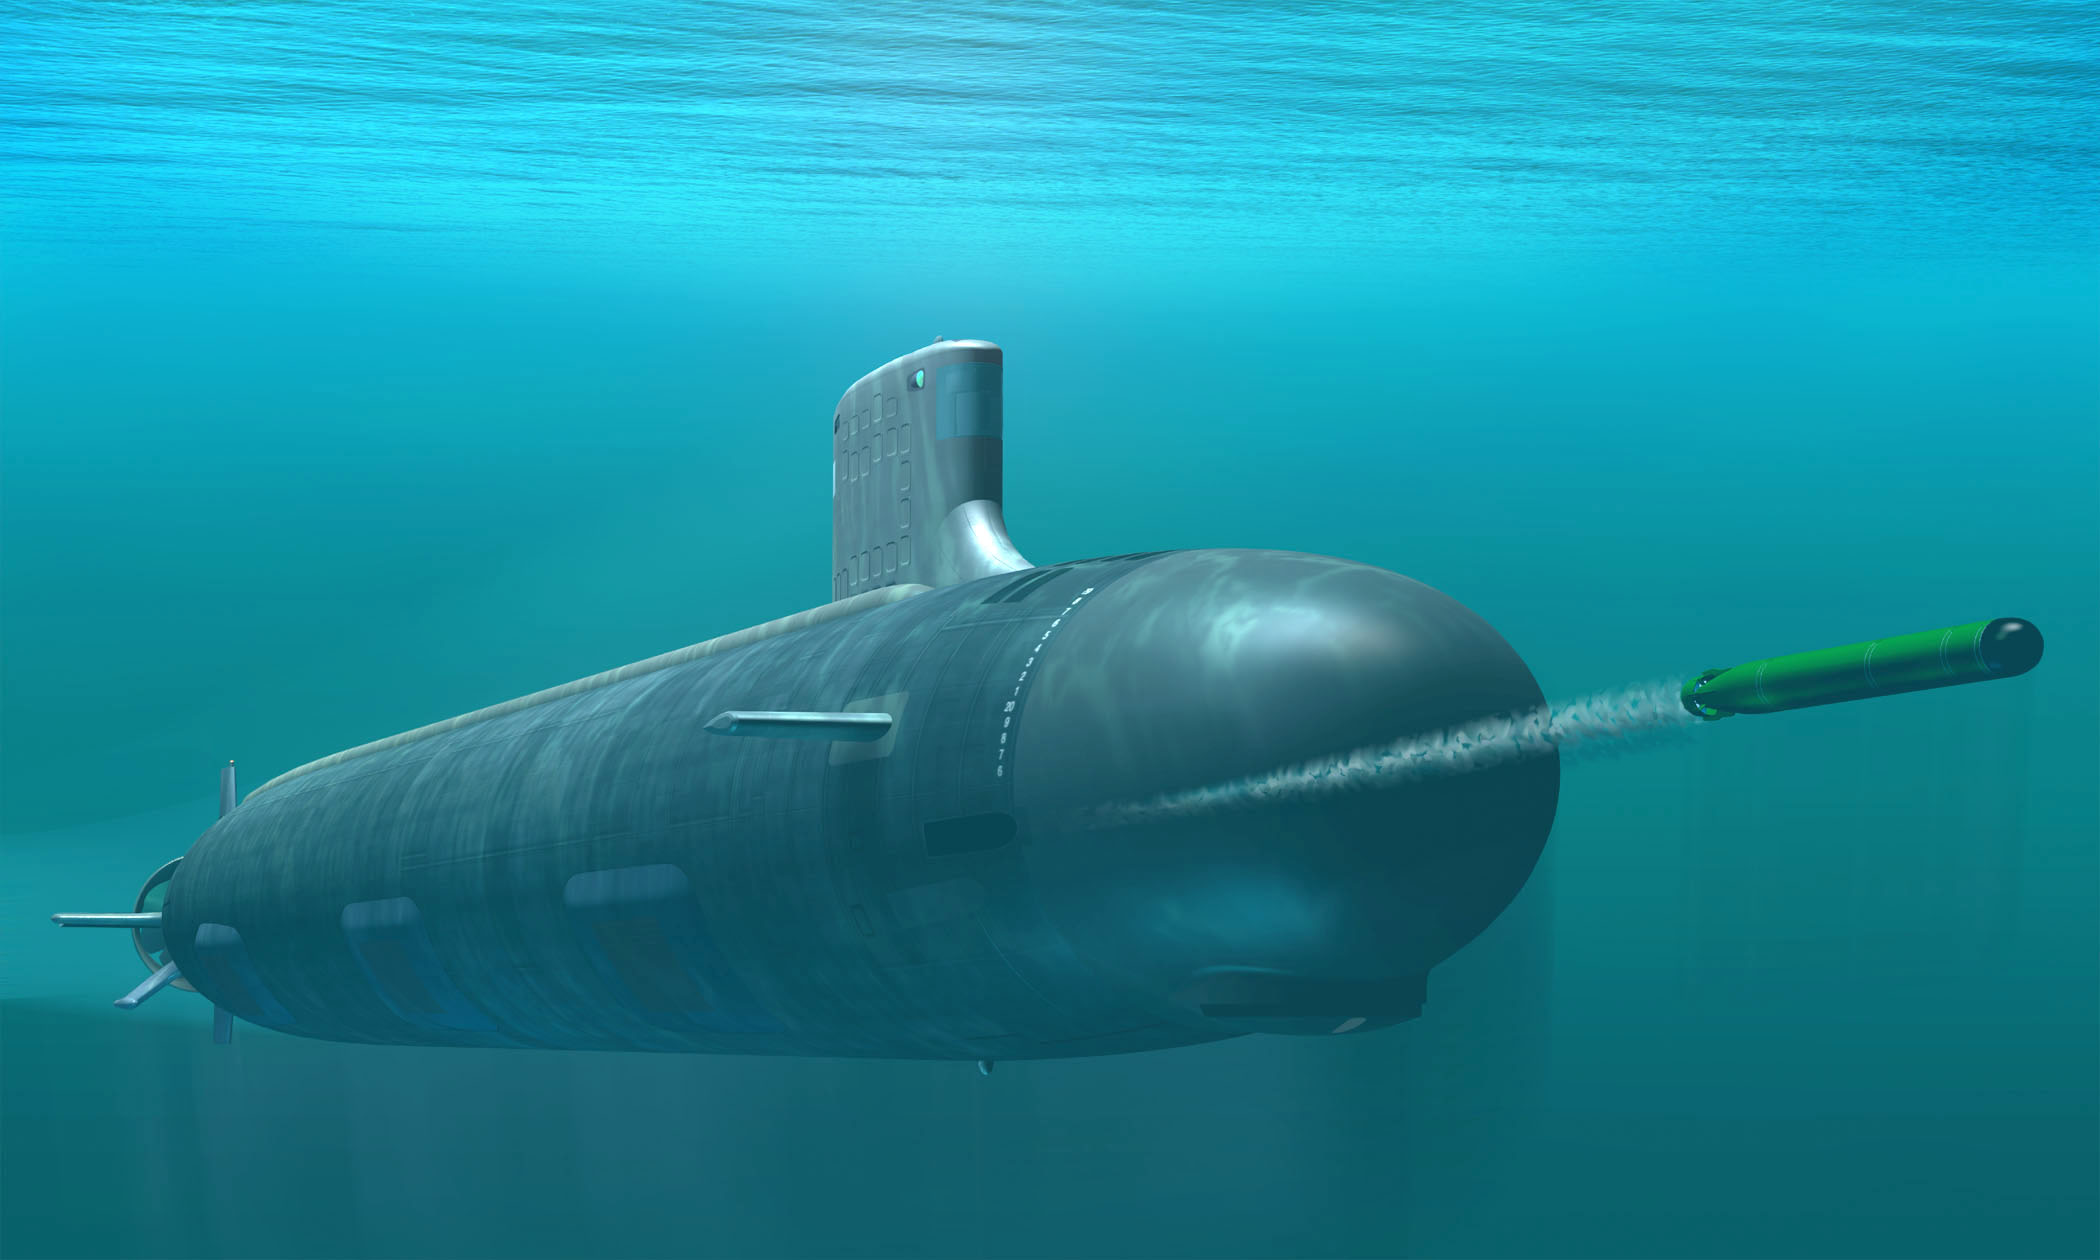
\includegraphics[height=8cm]{img/Virginia_class_submarine.jpg} 
			\caption{Illustration d'un sous-marin d'attaque, réalisé par Ron Stern}
		\end{figure}
		
		
	
		
		\vfill
		{\large \today \par}
	\end{titlepage}
	
	%	Page de garde
	%\maketitle
	\section*{Objectif du rapport}
	\begin{abstract}
	Afin de garantir la viabilité du projet avant d'investir dans des drones réels, notre client a fait l'acquisition d'un simulateur de drones. Le but est d'augmenter la vision des sous-marins d’attaque dans leurs environnement par l’intermédiaire de drones autonomes aériens.  Le développement du produit nécessite une collaboration avec nos clients pour permettre notre équipe de s’initier au domaine naval. Pour que notre équipe puisse se familiariser au domaine naval, il est essentiel de travailler en étroite collaboration avec nos clients tout au long du développement du produit. L'objectif de se rapport est de documenter le produit livrable selon l'analyse des besoins pour faciliter sa maintenance et son déploiement.  
\end{abstract}
	
	
	%fin page de garde 
	%\newpage
	
	%Sommaire
	\tableofcontents
	
	
	
	
	\section{Présentation des membres du groupe}
	
	\begin{figure}[h]
		\centering
		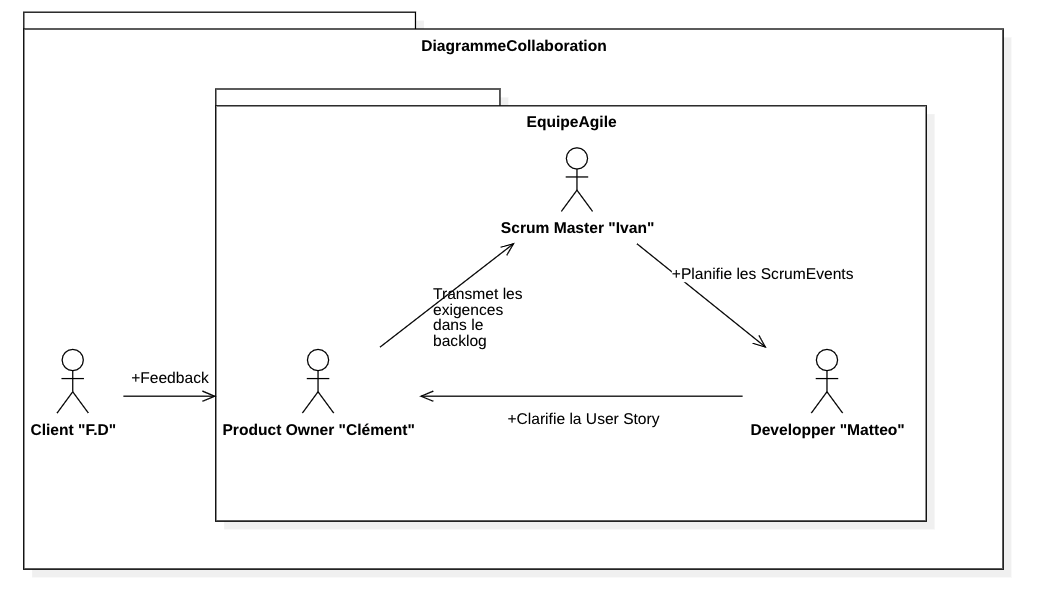
\includegraphics[height=8cm]{img/diagCollaboration.png} 
		\caption{Illustration de l'attribution des rôles principaux au sein de l'équipe.}
	\end{figure}
	
	\section{Exigences fonctionnelles (listes par catégorie)}
	
\subsection{Interface}
\begin{itemize}
	\item Le Logiciel doit être séparé entre un serveur et des clients
\end{itemize}

%	\hrulefill

\subsection{Serveur}
\begin{itemize}
	\item Le serveur doit posséder un éditeur de situation (EdS).
	\item Le serveur doit simuler la situation
	\item Le serveur doit offrir une vue 'replay' des résultat clients
\end{itemize}



\subsection{Editeur de situation (EdS)}
\begin{itemize}
	\item L'EdS doit permettre de créer ou modifier une situation.
	\item L'EdS doit permettre d'ajouter des obstacles OPFOR\footnote{Toute force ennemie: drônes, navires} à une situation.
	\item L'EdS doit permettre de définir une carte topographique de la situation.
	\item L'EdS doit permettre de définir un ou plusieurs points de départ pour les sous-marins de la situation.
	\item L'EdS doit permettre de définir un ou plusieurs objectifs à la situation.
\end{itemize}

\subsection{Une situation}
\begin{itemize}
	\item La situation doit pouvoir contenir des unités OPFOR.
	\item La situation doit contenir une carte topographique.
	\item La situation doit contenir un ou plusieurs points de départ pour les sous-marins de la situation.
	\item La situation doit contenir un ou plusieurs objectifs.
\end{itemize}


\subsection{Simulation}

Chaque objectif doit être assigné à un sous-marin uniquement.

\begin{itemize}
	\item La simulation doit être jouée sur le serveur.
	\item La simulation doit avoir ses sous-marins contrôlés par les clients.
\end{itemize}

%	\hrulefill

\subsection{OPFOR (forces ennemies)}
\begin{itemize}
	\item L'OPFOR doit avoir des unités anti-aériennes.
	\item L'OPFOR doit avoir des unités navales capables de se déplacer durant la situation.
	\item L'OPFOR doit avoir des unités autres pour les objectifs de reconnaissance.
\end{itemize}
%	\hrulefill

\subsection{Les unités}
\begin{itemize}
	\item Les unités AA OPFOR doivent pouvoir détecter les drones BLUFOR\footnote{Tout ce qui est unité allié :  les sous-marins, les drones...}.
	\item Les unités AA OPFOR doivent pouvoir détruire les drones BLUFOR.
\end{itemize}


\subsection{La vision}	
\begin{itemize}
	\item La vision replay doit offrir une vue BLUFOR de la situation.
	\item La vision replay doit offrir une vue omnisciente de la situation.
\end{itemize}

%	\hrulefill

\subsection{Le client}
Concernant le client : 
\begin{itemize}
	\item Le client doit planifier une résolution de la situation pour son sous-marin.
	\item Le client doit gérer un sous-marin et sa flotte de drones.
	\item Le client doit pouvoir contrôler le sous-marin.
	\item Le client doit afficher ce que son sous-marin voit.
	\item Le client doit afficher ce que ses drones à portée voient.
\end{itemize}

%\hrulefill

\subsection{Les drones}
\begin{itemize}
	\item Les drones doivent pouvoir patrouiller autour du sous-marin.
	\item Les drones doivent pouvoir faire de la reconnaissance.
	\item Les drones doivent pouvoir faire des missions de reconnaissance autonomes.
	\item Les drones doivent pouvoir faire garde en autonomie.
	\item Les drones doivent pouvoir être contrôlés par le client.
	\item Les drones doivent envoyer des rapports de détection à la base de données.
\end{itemize}

La base de données doit contenir des informations sur les drones.

\subsection{Les sous-marins}
\begin{itemize}
	\item Le sous-marin doit pouvoir changer de profondeur.
	\item Le sous-marin doit pouvoir communiquer avec ses drones.
	\item Le sous-marin doit pouvoir communiquer avec son commandement.
\end{itemize}

	
	\section{Maquettage du produit}
	%\input{file}
	
	\section{Conception UML}
		\subsection{Axe fonctionnel}



\subsubsection{Diagramme de cas d'usage SI Serveur}
\begin{figure}[H]
	\centering
	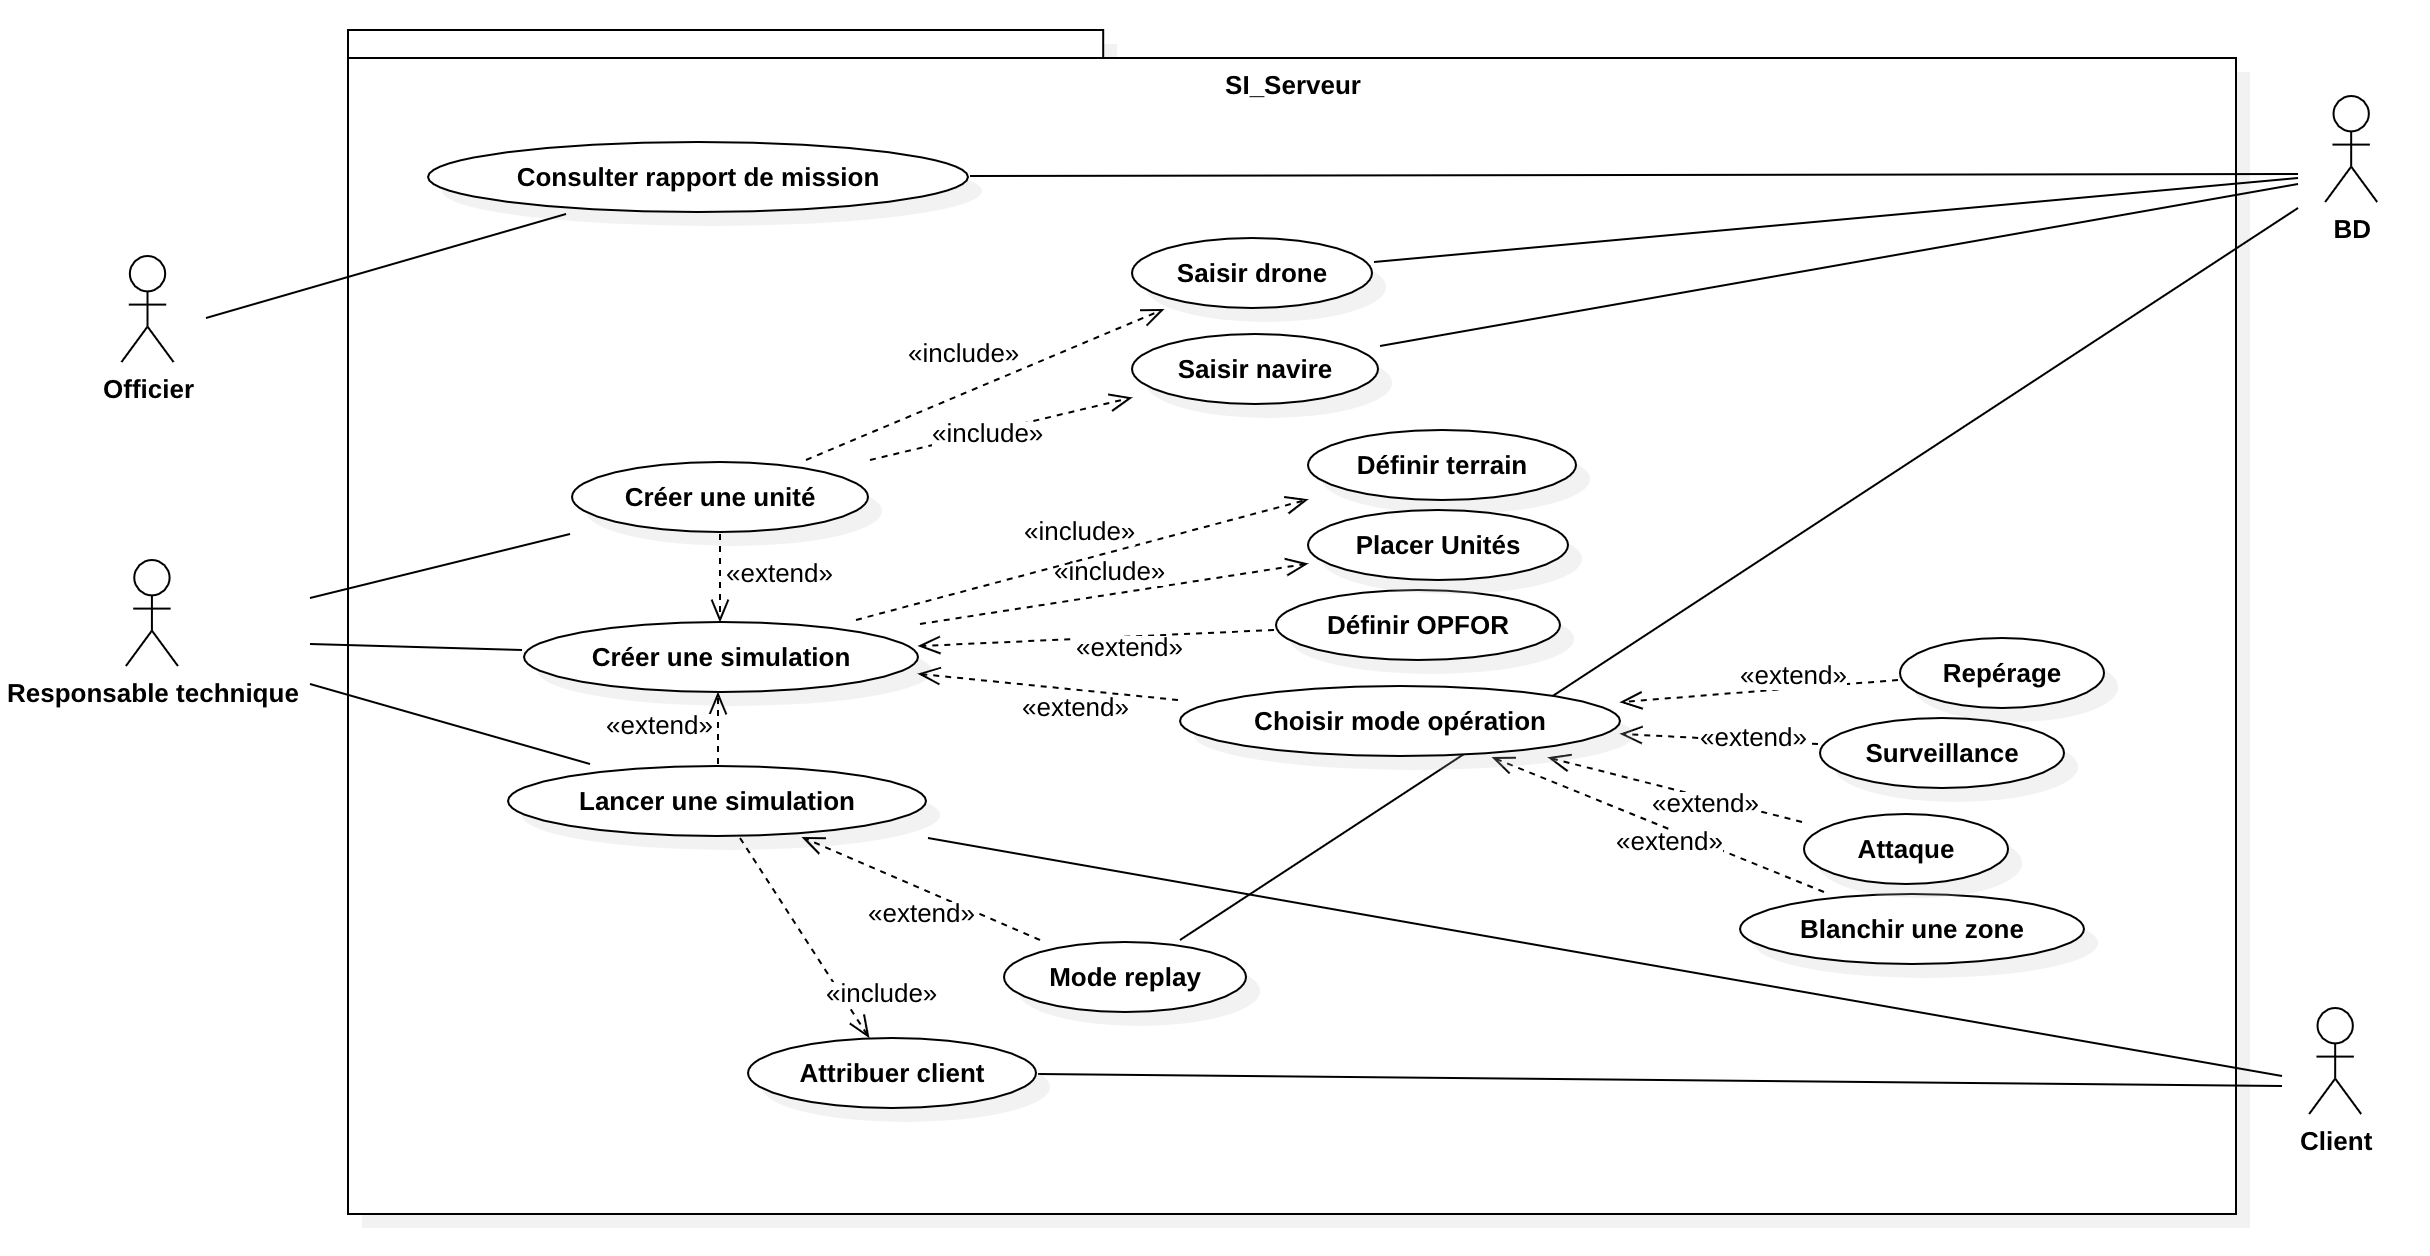
\includegraphics[height=8cm]{img/CUSI_Serveur.png} 
	\caption{CU SI Serveur.}
\end{figure}
\subsubsection{Diagramme de cas d'usage SI Client}
\begin{figure}[H]
	\centering
	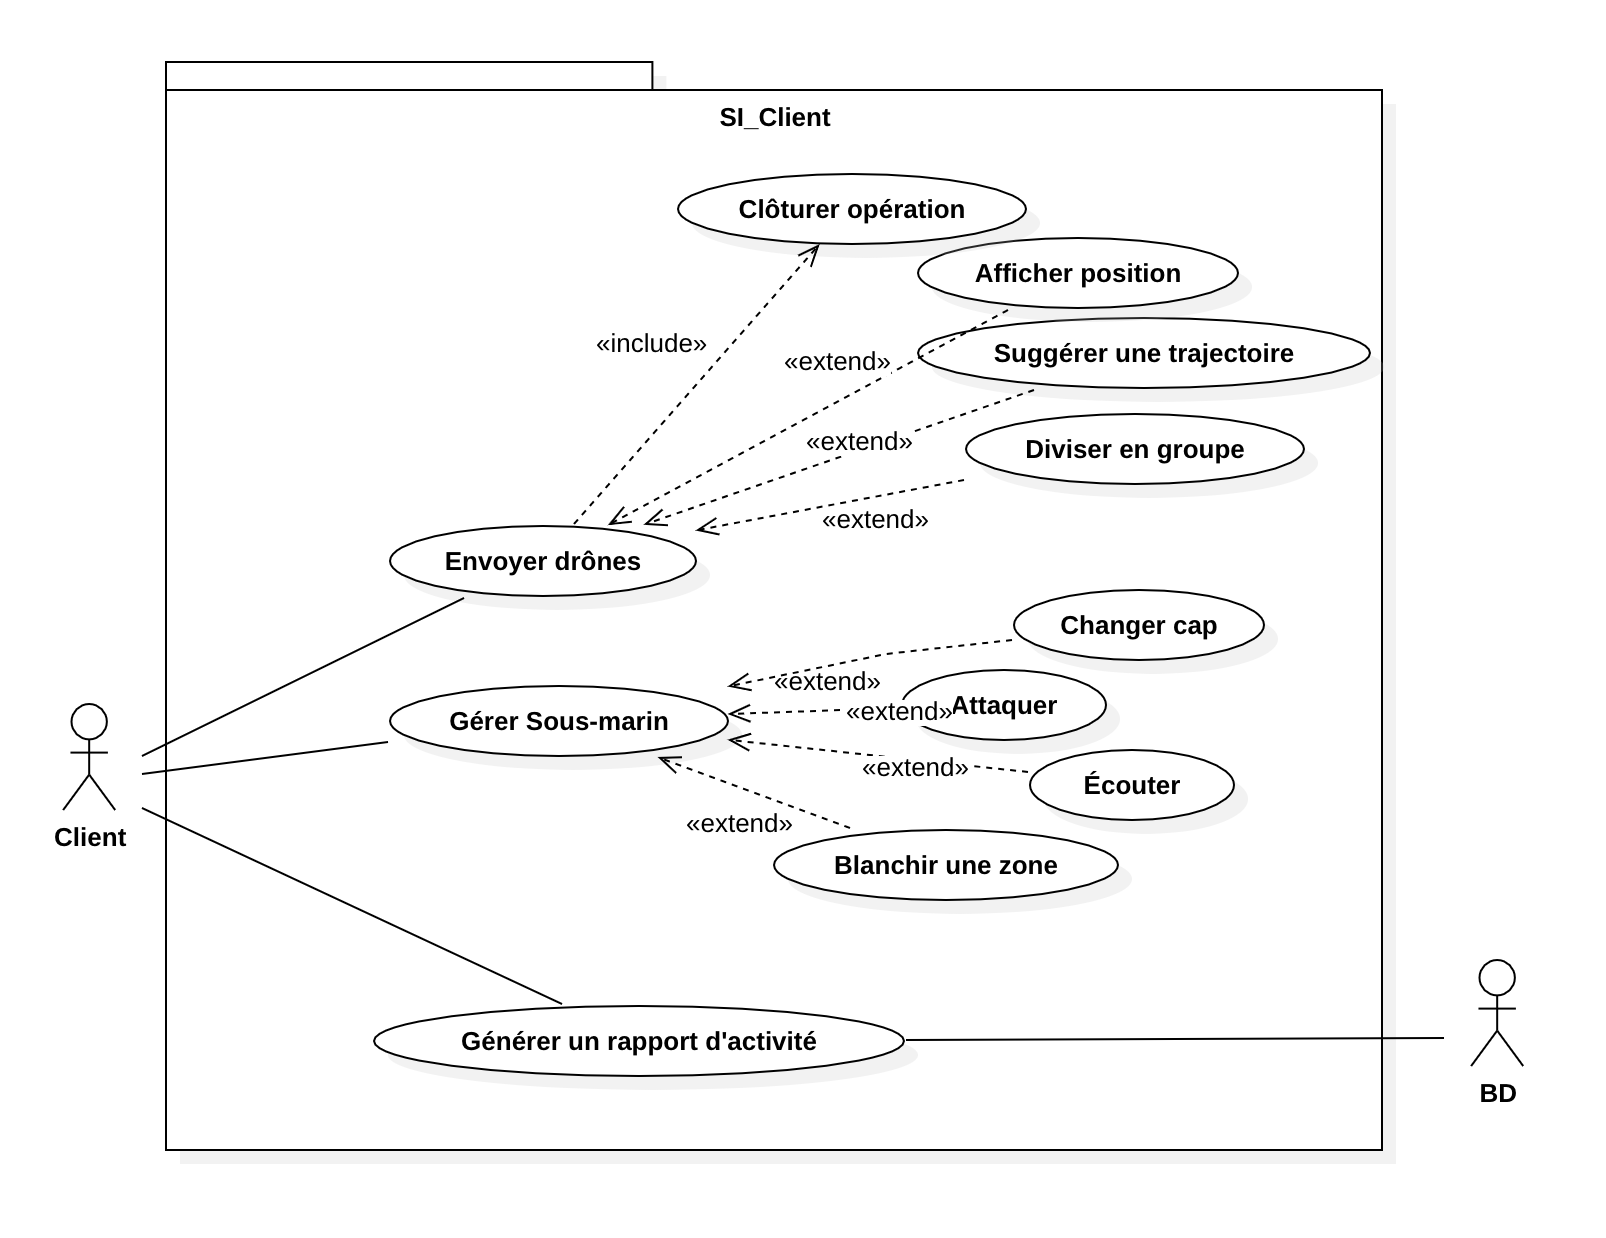
\includegraphics[height=8cm]{img/CUSI_Client.png} 
	\caption{CU SI Client.}
\end{figure}


\subsubsection{Structure du système niveau 1}
\begin{figure}[H]
	\centering
	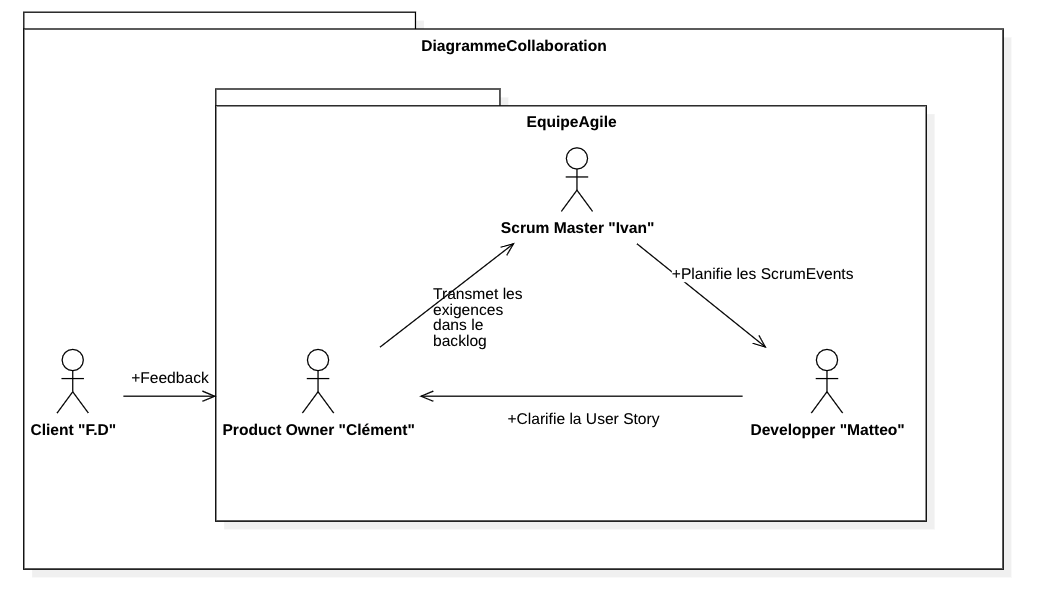
\includegraphics[height=8cm]{img/diagCollaboration.png} 
	\caption{Illustration de l'attribution des rôles principaux au sein de l'équipe.}
\end{figure}

\subsubsection{Structure du système niveau 2}
\begin{figure}[H]
	\centering
	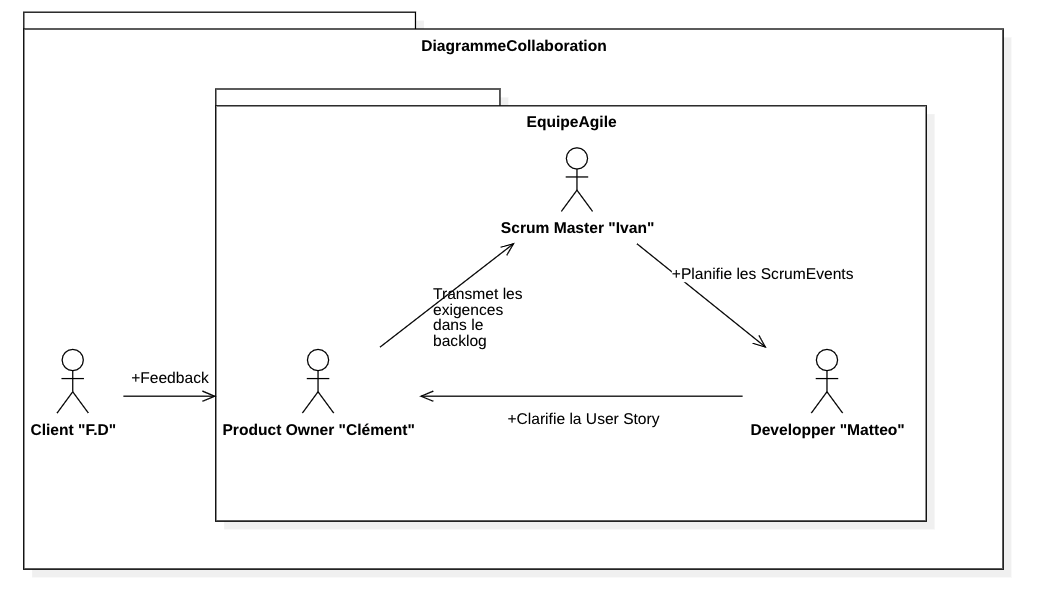
\includegraphics[height=8cm]{img/diagCollaboration.png} 
	\caption{Illustration de l'attribution des rôles principaux au sein de l'équipe.}
\end{figure}


\subsection{Axe statique}
\subsubsection{Diagramme des classes partie Serveur}
\begin{figure}[H]
	\centering
	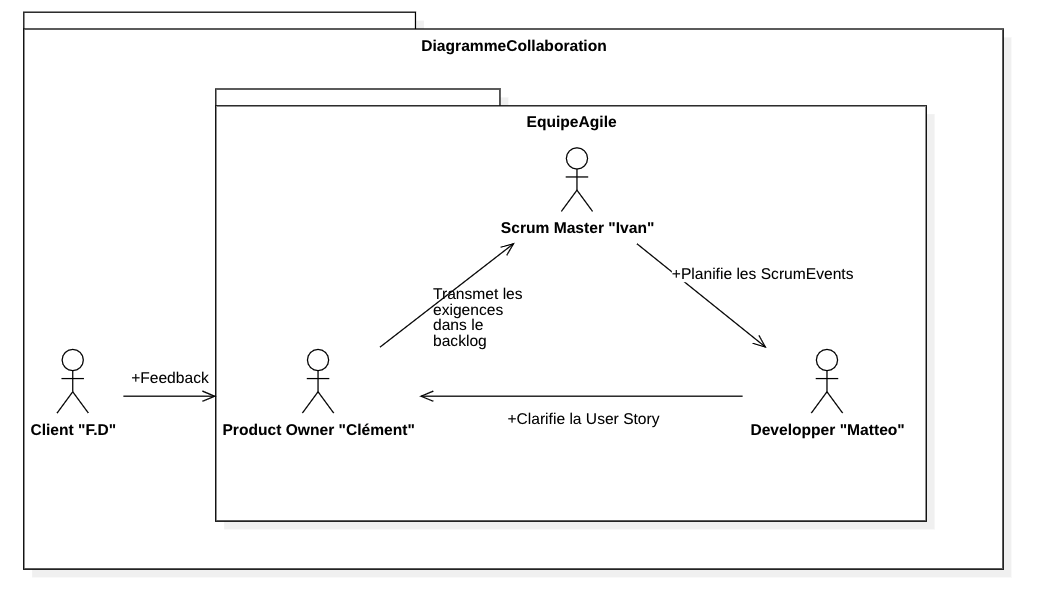
\includegraphics[height=8cm]{img/diagCollaboration.png} 
	\caption{Illustration de l'attribution des rôles principaux au sein de l'équipe.}
\end{figure}

\subsubsection{Diagramme des classes partie Client}
\begin{figure}[H]
	\centering
	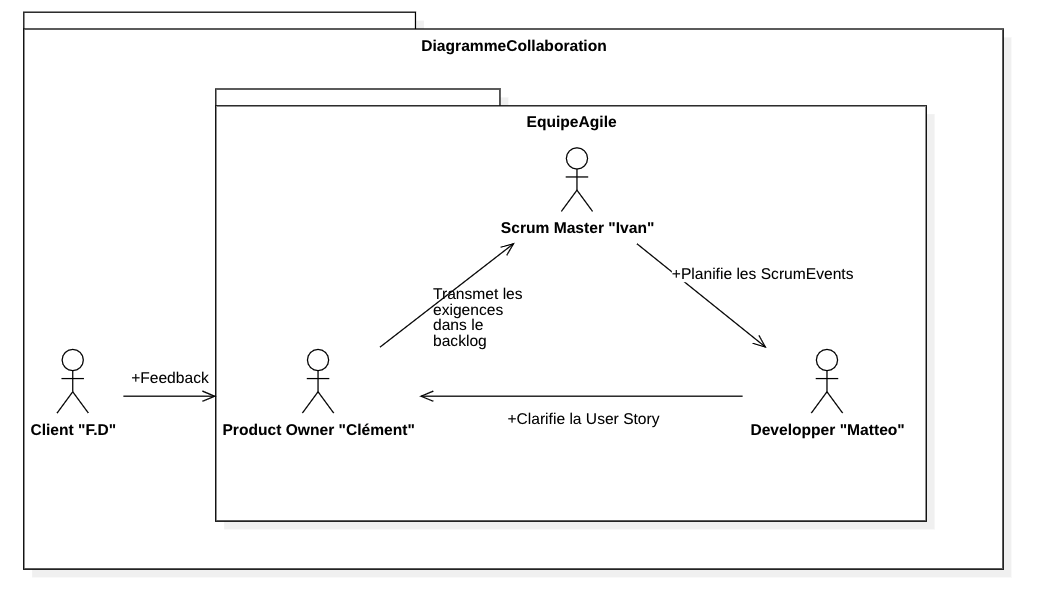
\includegraphics[height=8cm]{img/diagCollaboration.png} 
	\caption{Illustration de l'attribution des rôles principaux au sein de l'équipe.}
\end{figure}


\subsection{Axe dynamique}
\subsubsection{Diagramme de séquence Client-Serveur}
\begin{figure}[H]
	\centering
	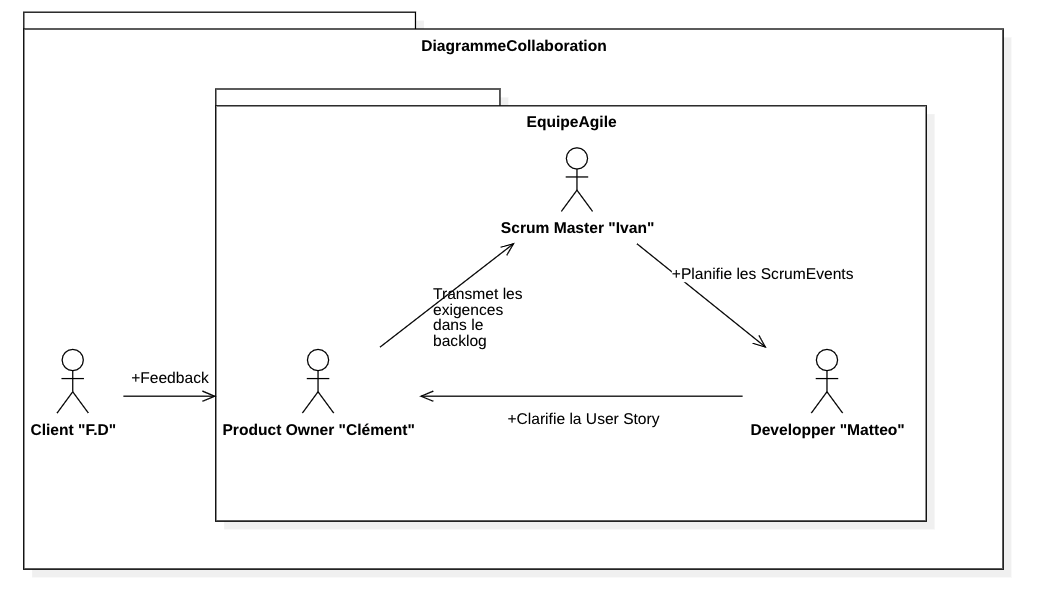
\includegraphics[height=8cm]{img/diagCollaboration.png} 
	\caption{Illustration de l'attribution des rôles principaux au sein de l'équipe.}
\end{figure}

	
	\section{Le manuel d’installation du logiciel}
	 %\input{file}
	 
	 \section{Le manuel utilisateur du logiciel}
	 %\input{file}
	 
	 \section{Le planning mis en œuvre durant le projet}
	 

\subsection{Sprint 1}

		\subsubsection{Sprint Planning  | 27 février 2024}
		\begin{enumerate}
			\item Liste de l’ensemble des demandes du client.
			\item Cadrage initial du projet et définition des objectifs; pour se faire : réflexion avec l'équipe et le représentant du client pour se familiariser avec le domaine du produit.
		\end{enumerate}
		
		\subsubsection*{Tâches à réaliser}
		\begin{itemize}
			\item Définition des besoins : surveillance, renseignement, reconnaissance.
			\item Schématisation du navires et de ses drones.
			\item Familiarisation avec la doctrine detection passive.
			\item Prise en compte de la dimension distribution serveur/client pour simuler les échanges entre les systèmes.
			\item Prototype papier d’une base de données pour contenir les rapports de détection, les caractéristiques des drones et l’état des missions.
		\end{itemize}
		
		\subsubsection{Daily Scrum du 12 Mars 2024}
		\subsubsection*{Objectif(s)}
		\begin{itemize}
			\item Liste de l’ensemble des demandes et prise en compte des retours du client.
		\end{itemize}
		
		\subsubsection*{Tâches réalisées}
		\begin{itemize}
			\item Listes des exigences fonctionnelles.
			\item Échange entre le client, son représentant pour éclaircir les zones de flou sur le fonctionnement du système et lever des barrières et des interrogations autour des différents usages du système à travers d’un schéma et d’échanges.
		\end{itemize}



\subsection{Sprint 2}
	
	\subsubsection{Sprint planning | 19 Mars 2024}
	\subsubsection*{Objectif(s)}
	\begin{itemize}
		\item Définitions des objectifs à réaliser entre l’équipe et les représentants du client.
		\item Planification des tâches.
	\end{itemize}
	
	\subsubsection*{Tâches réalisées}
	\begin{itemize}
		\item Réalisation du diagramme de cas d’usage.
		\item Liste des différentes fonctions pour chaque mode du simulateur.
		\item Définition des contraintes du système et de son articulation.
	\end{itemize}
	
	\subsubsection{Sprint Review du 26 mars 2024}
	
	\subsubsection*{Tâches réalisées}
	\begin{itemize}
		\item Réalisation du diagramme statique (objet).
		\item Assimilation des rôles pour la méthode Agile Scrum.
		\item Recherche de développement du code : PyQT ou Tkinter.
	\end{itemize}
	
	\subsubsection{Daily Scrum | 8 Avril 2024}
	\subsubsection*{Objectif(s)}
	\begin{itemize}
		\item Clarification de ce qui a été réalisé, des différentes tâches à finaliser et démarrage d’un cycle extreme programming.
	\end{itemize}
	
	\subsubsection*{Tâches réalisées}
	\begin{itemize}
		\item Échange au tableau sur la conception IHM de notre simulateur.
		\item Développement en binôme : Clément pour la partie serveur et Mattéo pour la maquette de l’interface. Programmation modulaire avec Tkinter en Python3.
		\item Réalisation et reprise des diagrammes UML.
	\end{itemize}
	
	\subsubsection{Sprint Review | 16 Avril 2024}
	\subsubsection*{Objectif(s)}
	\begin{itemize}
		\item Vérification du code et remise en question du développement.
	\end{itemize}
	
	\subsubsection*{Tâches réalisées}
	\begin{itemize}
		\item Ajustement de l’IHM à partir de la maquette.
		\item Échange avec le client pour réviser l’approche client-serveur.
	\end{itemize}
	
	\subsubsection{Sprint Retrospective 1 | 23 Avril 2024}
	\subsubsection*{Objectif(s)}
	\begin{itemize}
		\item Clarification de ce qui a été réalisé.
		\item Reprise des diagrammes UML.
		\item Développement des classes selon le MVC.
	\end{itemize}
	
	\subsubsection{Sprint Retrospective 2 | 29 Avril 2024}
	\subsubsection*{Clarifications}
	\begin{itemize}
		\item Briefing sur ce qui a été réalisé.
		\item Réalisation d'un diagramme de Gantt.
		\item Réalisation d'un diagramme de séquence dynamique
		\item Vérification du code selon le modèle UML.
	\end{itemize}
	
	



\section{Diagramme de Gantt}

\subsection*{29 Avril 2024}
\begin{figure}[H]
	\centering
	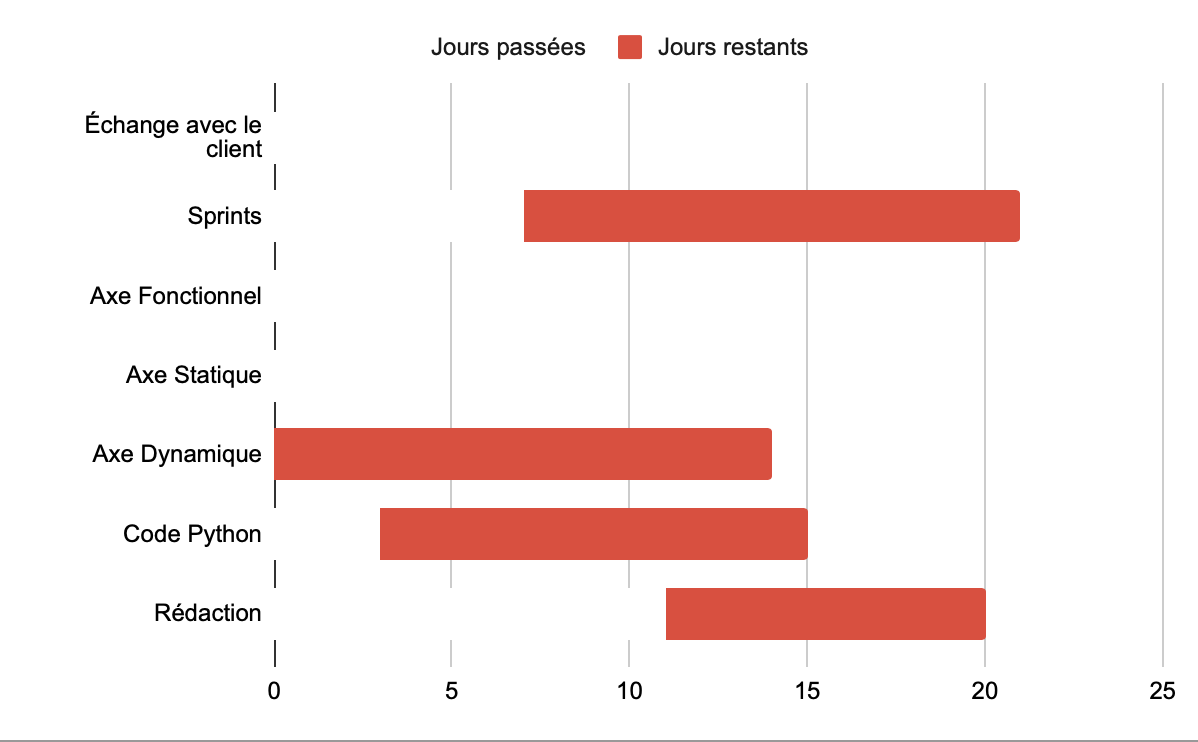
\includegraphics[height=8cm]{img/gantt_290424.png}
	\caption{Diagramme de Gantt le 29 Avril 2024}
\end{figure}

\begin{table}[H]
	\centering
	\caption{Planning du Projet}
	\begin{tabular}{
			>{\columncolor[HTML]{C0C0C0}}l |r|r|r|r|}
		\cline{2-5}
		\cellcolor[HTML]{EFEFEF}                                             & \multicolumn{1}{l|}{\cellcolor[HTML]{C0C0C0}Date de début} & \multicolumn{1}{l|}{\cellcolor[HTML]{C0C0C0}Jours passées} & \multicolumn{1}{l|}{\cellcolor[HTML]{C0C0C0}Jours restants} & \multicolumn{1}{l|}{\cellcolor[HTML]{C0C0C0}TOTAL} \\ \hline
		\multicolumn{1}{|l|}{\cellcolor[HTML]{C0C0C0}Échange avec le client} & 27/02/2024                                                 & 3                                                          & 0                                                           & 01/03/2024                                         \\ \hline
		\multicolumn{1}{|l|}{\cellcolor[HTML]{C0C0C0}Sprints}                & 27/02/2024                                                 & 7                                                          & 14                                                          & 19/03/2024                                         \\ \hline
		\multicolumn{1}{|l|}{\cellcolor[HTML]{C0C0C0}Axe Fonctionnel}        & 23/04/2024                                                 & 4                                                          & 0                                                           & 27/04/2024                                         \\ \hline
		\multicolumn{1}{|l|}{\cellcolor[HTML]{C0C0C0}Axe Statique}           & 19/03/2024                                                 & 3                                                          & 0                                                           & 22/03/2024                                         \\ \hline
		\multicolumn{1}{|l|}{\cellcolor[HTML]{C0C0C0}Axe Dynamique}          & 29/04/2024                                                 & 0                                                          & 14                                                          & 13/05/2024                                         \\ \hline
		\multicolumn{1}{|l|}{\cellcolor[HTML]{C0C0C0}Code Python}            & 29/04/2024                                                 & 3                                                          & 12                                                          & 14/05/2024                                         \\ \hline
		\multicolumn{1}{|l|}{\cellcolor[HTML]{C0C0C0}Rédaction}              & 05/03/2024                                                 & 11                                                         & 9                                                           & 15/05/2024                                         \\ \hline
	\end{tabular}
\end{table}

\subsection*{8 Mai 2024}
\begin{figure}[H]
	\centering
	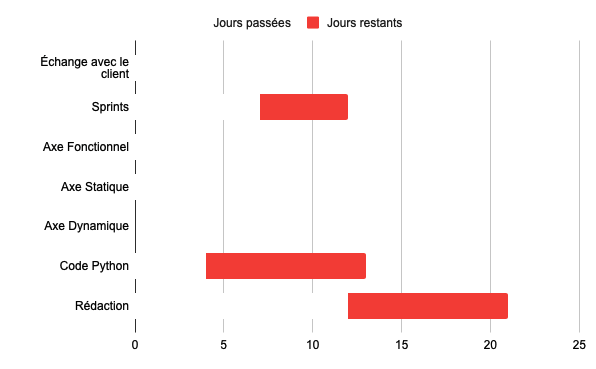
\includegraphics[height=8cm]{img/gantt_08052024.png}
	\caption{Diagramme de Gantt le 8 Mai 2024}
\end{figure}

% Please add the following required packages to your document preamble:
% \usepackage[table,xcdraw]{xcolor}
% Beamer presentation requires \usepackage{colortbl} instead of \usepackage[table,xcdraw]{xcolor}
% Please add the following required packages to your document preamble:
% \usepackage[table,xcdraw]{xcolor}
% Beamer presentation requires \usepackage{colortbl} instead of \usepackage[table,xcdraw]{xcolor}
\begin{table}[H]
	\begin{tabular}{
			>{\columncolor[HTML]{EFEFEF}}l |r|r|r|r|}
		\cline{2-5}
		& \multicolumn{1}{l|}{\cellcolor[HTML]{EFEFEF}Date de début} & \multicolumn{1}{l|}{\cellcolor[HTML]{EFEFEF}Jours passées} & \multicolumn{1}{l|}{\cellcolor[HTML]{EFEFEF}Jours restants} & \multicolumn{1}{l|}{\cellcolor[HTML]{EFEFEF}TOTAL} \\ \hline
		\multicolumn{1}{|l|}{\cellcolor[HTML]{EFEFEF}Échange avec le client} & 27/02/2024                                                 & 4                                                          & 0                                                           & 01/03/2024                                         \\ \hline
		\multicolumn{1}{|l|}{\cellcolor[HTML]{EFEFEF}Sprints}                & 27/02/2024                                                 & 7                                                          & 5                                                           & 19/03/2024                                         \\ \hline
		\multicolumn{1}{|l|}{\cellcolor[HTML]{EFEFEF}Axe Fonctionnel}        & 23/04/2024                                                 & 4                                                          & 0                                                           & 27/04/2024                                         \\ \hline
		\multicolumn{1}{|l|}{\cellcolor[HTML]{EFEFEF}Axe Statique}           & 19/03/2024                                                 & 3                                                          & 0                                                           & 22/03/2024                                         \\ \hline
		\multicolumn{1}{|l|}{\cellcolor[HTML]{EFEFEF}Axe Dynamique}          & 29/04/2024                                                 & 0                                                          & 0                                                           & 13/05/2024                                         \\ \hline
		\multicolumn{1}{|l|}{\cellcolor[HTML]{EFEFEF}Code Python}            & 29/04/2024                                                 & 4                                                          & 9                                                           & 17/05/2024                                         \\ \hline
		\multicolumn{1}{|l|}{\cellcolor[HTML]{EFEFEF}Rédaction}              & 05/03/2024                                                 & 12                                                         & 9                                                           & 17/05/2024                                         \\ \hline
	\end{tabular}
\end{table}

\subsection*{Bilan de la méthode Agile}
Nous avons pu rectifier le livrable que nous allons fournir en un seul logiciel, en deux logiciels distincts (client et serveur). Ces améliorations ont été discutées lors des échanges, tout comme la création d’une interface graphique pour la partie client alors que nous pensions plutôt à une interaction par commande via un terminal.  

	 
	
	
\end{document}